\documentclass[11pt]{beamer}
\usepackage{amsmath}

\usetheme{CambridgeUS}
\usecolortheme{dolphin}
\setbeamertemplate{caption}[numbered]
\setbeamerfont{title}{size=\large}
\setbeamerfont{author}{size=\small}
\setbeamerfont{date}{size=\small}
\setbeamerfont{institute}{size=\small}
\titlegraphic{
  \parbox{0.9\linewidth}{
    \centering
    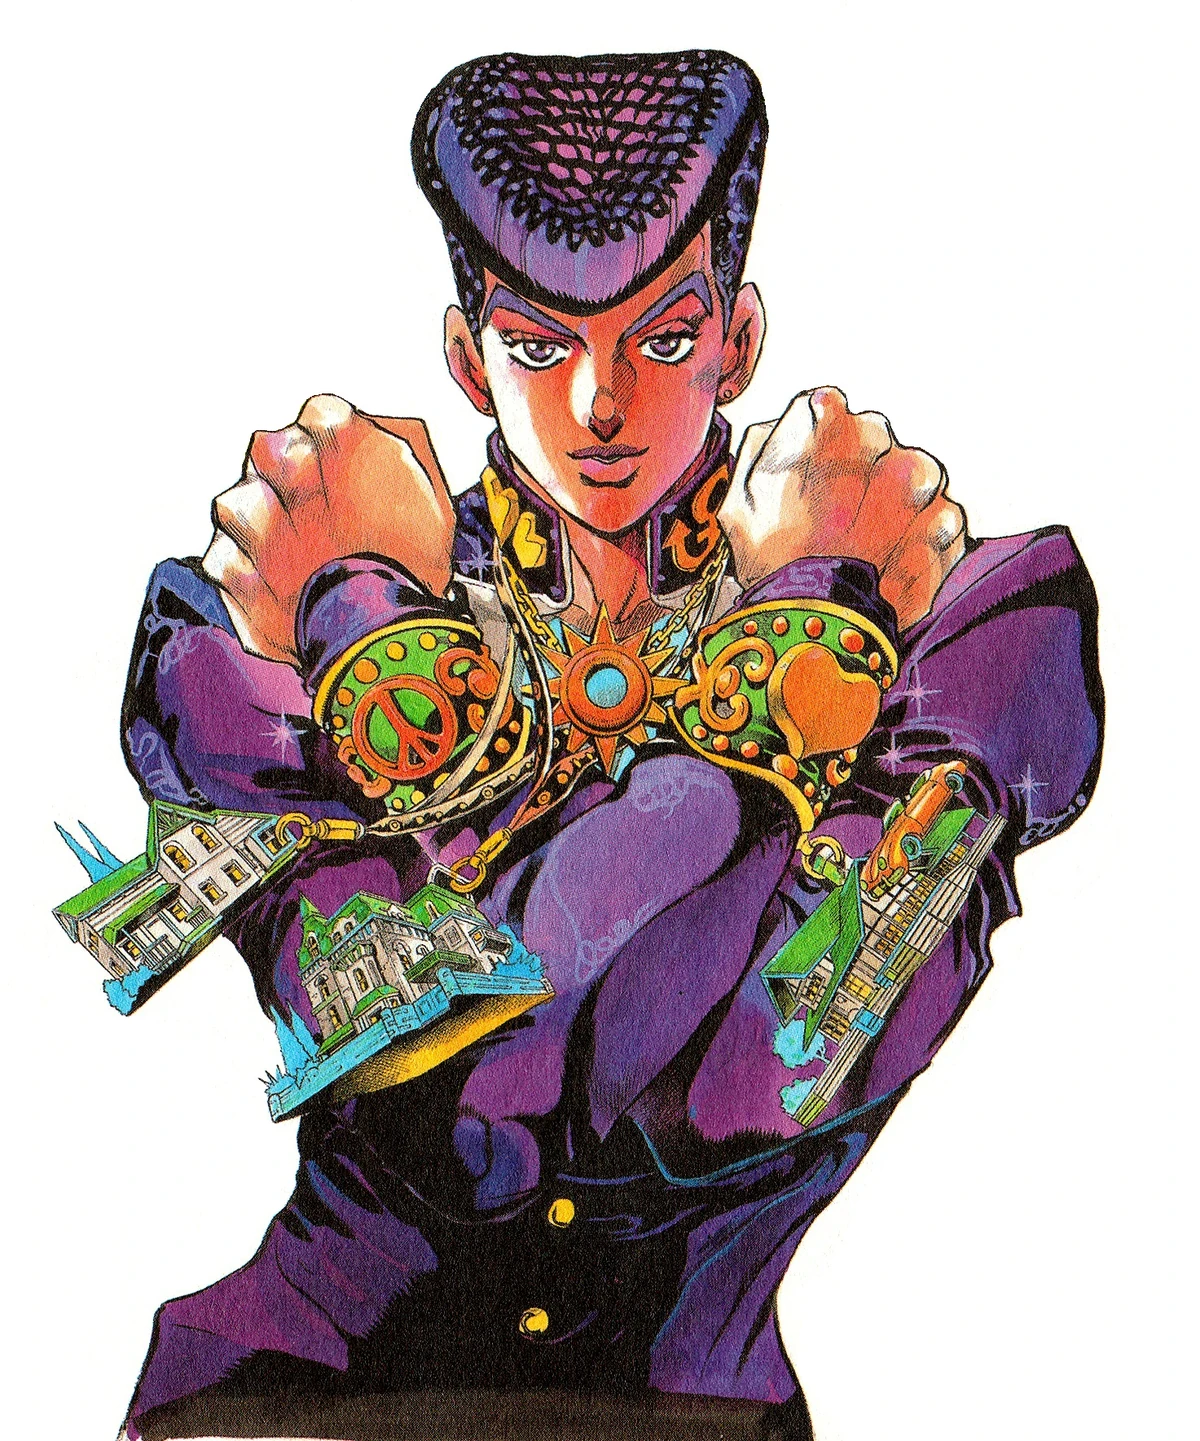
\includegraphics[height=3.5cm]{imagen/jojo.png}\\
    \scriptsize Josuke Higashikata, por Hirohiko Araki
  }
}


\title{Actividad Semanal 2}
\author{Iago Hernández Bautista}
\institute[]{Facultad de Ciencias}
\date[\today]{\today}

\begin{document}

\begin{frame}
  \titlepage
\end{frame}

\begin{frame}{Teorema del binomio \cite{mate}}
  Para cualquier entero positivo n, se tiene que:
  \[
  \displaystyle
  (a+b)^n = \sum_{k=0}^n \binom{n}{k} a^{n-k} b^k
  \]
  Este teorema pertenece a la sección de conteo (según el libro que consulté). Lo escogí porque mi maestro lo usaba bastante en CCH aunque nunca lo explicó.
\end{frame}

\begin{frame}{Resolver la ecuación}
  \begin{align*}
    (3/4) * x + 9 &= 15\\
    (3/4) * x + 9 - 9 &= 15 - 9\\
    (3/4) * x &= 6\\
    4 * (3/4) * x &= 4 * 6\\
    (12/4) * x &= 24\\
    3x &= 24\\
    3x / 3 &= 24 / 3\\
    x &= 8\\
  \end{align*}  
\end{frame}

\begin{frame}[allowframebreaks]
  \frametitle{Bibliografia}
  \bibliographystyle{plainnat}
  \bibliography{Referencias}
\end{frame}

\end{document}
